\documentclass[12pt,ignorenonframetext,]{beamer}
\setbeamertemplate{caption}[numbered]
\setbeamertemplate{caption label separator}{: }
\setbeamercolor{caption name}{fg=normal text.fg}
\beamertemplatenavigationsymbolsempty
\usepackage{lmodern}
\usepackage{amssymb,amsmath}
\usepackage{ifxetex,ifluatex}
\usepackage{fixltx2e} % provides \textsubscript
\ifnum 0\ifxetex 1\fi\ifluatex 1\fi=0 % if pdftex
\usepackage[T1]{fontenc}
\usepackage[utf8]{inputenc}
\else % if luatex or xelatex
\ifxetex
\usepackage{mathspec}
\else
\usepackage{fontspec}
\fi
\defaultfontfeatures{Ligatures=TeX,Scale=MatchLowercase}
\fi
% use upquote if available, for straight quotes in verbatim environments
\IfFileExists{upquote.sty}{\usepackage{upquote}}{}
% use microtype if available
\IfFileExists{microtype.sty}{%
\usepackage{microtype}
\UseMicrotypeSet[protrusion]{basicmath} % disable protrusion for tt fonts
}{}
\newif\ifbibliography
\usepackage{color}
\usepackage{fancyvrb}
\newcommand{\VerbBar}{|}
\newcommand{\VERB}{\Verb[commandchars=\\\{\}]}
\DefineVerbatimEnvironment{Highlighting}{Verbatim}{commandchars=\\\{\}}
% Add ',fontsize=\small' for more characters per line
\usepackage{framed}
\definecolor{shadecolor}{RGB}{248,248,248}
\newenvironment{Shaded}{\begin{snugshade}}{\end{snugshade}}
\newcommand{\KeywordTok}[1]{\textcolor[rgb]{0.13,0.29,0.53}{\textbf{{#1}}}}
\newcommand{\DataTypeTok}[1]{\textcolor[rgb]{0.13,0.29,0.53}{{#1}}}
\newcommand{\DecValTok}[1]{\textcolor[rgb]{0.00,0.00,0.81}{{#1}}}
\newcommand{\BaseNTok}[1]{\textcolor[rgb]{0.00,0.00,0.81}{{#1}}}
\newcommand{\FloatTok}[1]{\textcolor[rgb]{0.00,0.00,0.81}{{#1}}}
\newcommand{\ConstantTok}[1]{\textcolor[rgb]{0.00,0.00,0.00}{{#1}}}
\newcommand{\CharTok}[1]{\textcolor[rgb]{0.31,0.60,0.02}{{#1}}}
\newcommand{\SpecialCharTok}[1]{\textcolor[rgb]{0.00,0.00,0.00}{{#1}}}
\newcommand{\StringTok}[1]{\textcolor[rgb]{0.31,0.60,0.02}{{#1}}}
\newcommand{\VerbatimStringTok}[1]{\textcolor[rgb]{0.31,0.60,0.02}{{#1}}}
\newcommand{\SpecialStringTok}[1]{\textcolor[rgb]{0.31,0.60,0.02}{{#1}}}
\newcommand{\ImportTok}[1]{{#1}}
\newcommand{\CommentTok}[1]{\textcolor[rgb]{0.56,0.35,0.01}{\textit{{#1}}}}
\newcommand{\DocumentationTok}[1]{\textcolor[rgb]{0.56,0.35,0.01}{\textbf{\textit{{#1}}}}}
\newcommand{\AnnotationTok}[1]{\textcolor[rgb]{0.56,0.35,0.01}{\textbf{\textit{{#1}}}}}
\newcommand{\CommentVarTok}[1]{\textcolor[rgb]{0.56,0.35,0.01}{\textbf{\textit{{#1}}}}}
\newcommand{\OtherTok}[1]{\textcolor[rgb]{0.56,0.35,0.01}{{#1}}}
\newcommand{\FunctionTok}[1]{\textcolor[rgb]{0.00,0.00,0.00}{{#1}}}
\newcommand{\VariableTok}[1]{\textcolor[rgb]{0.00,0.00,0.00}{{#1}}}
\newcommand{\ControlFlowTok}[1]{\textcolor[rgb]{0.13,0.29,0.53}{\textbf{{#1}}}}
\newcommand{\OperatorTok}[1]{\textcolor[rgb]{0.81,0.36,0.00}{\textbf{{#1}}}}
\newcommand{\BuiltInTok}[1]{{#1}}
\newcommand{\ExtensionTok}[1]{{#1}}
\newcommand{\PreprocessorTok}[1]{\textcolor[rgb]{0.56,0.35,0.01}{\textit{{#1}}}}
\newcommand{\AttributeTok}[1]{\textcolor[rgb]{0.77,0.63,0.00}{{#1}}}
\newcommand{\RegionMarkerTok}[1]{{#1}}
\newcommand{\InformationTok}[1]{\textcolor[rgb]{0.56,0.35,0.01}{\textbf{\textit{{#1}}}}}
\newcommand{\WarningTok}[1]{\textcolor[rgb]{0.56,0.35,0.01}{\textbf{\textit{{#1}}}}}
\newcommand{\AlertTok}[1]{\textcolor[rgb]{0.94,0.16,0.16}{{#1}}}
\newcommand{\ErrorTok}[1]{\textcolor[rgb]{0.64,0.00,0.00}{\textbf{{#1}}}}
\newcommand{\NormalTok}[1]{{#1}}
\usepackage{graphicx,grffile}
\makeatletter
\def\maxwidth{\ifdim\Gin@nat@width>\linewidth\linewidth\else\Gin@nat@width\fi}
\def\maxheight{\ifdim\Gin@nat@height>\textheight0.8\textheight\else\Gin@nat@height\fi}
\makeatother
% Scale images if necessary, so that they will not overflow the page
% margins by default, and it is still possible to overwrite the defaults
% using explicit options in \includegraphics[width, height, ...]{}
\setkeys{Gin}{width=\maxwidth,height=\maxheight,keepaspectratio}

% Prevent slide breaks in the middle of a paragraph:
\widowpenalties 1 10000
\raggedbottom

\AtBeginPart{
\let\insertpartnumber\relax
\let\partname\relax
\frame{\partpage}
}
\AtBeginSection{
\ifbibliography
\else
\let\insertsectionnumber\relax
\let\sectionname\relax
\frame{\sectionpage}
\fi
}
\AtBeginSubsection{
\let\insertsubsectionnumber\relax
\let\subsectionname\relax
\frame{\subsectionpage}
}

\setlength{\parindent}{0pt}
\setlength{\parskip}{6pt plus 2pt minus 1pt}
\setlength{\emergencystretch}{3em}  % prevent overfull lines
\providecommand{\tightlist}{%
\setlength{\itemsep}{0pt}\setlength{\parskip}{0pt}}
\setcounter{secnumdepth}{0}

\title{BIOST 311: Assumptions and diagnostics for linear regression}
\author{Arjun Sondhi}
\date{4/25/2018}

\begin{document}
\frame{\titlepage}

\begin{frame}{Linear regression model}

Recall the form of the (multiple) linear regression model:

\[
\begin{aligned}
E[Y_i \mid X_{i1}, \dots, X_{ip}] &= \beta_0 + \beta_1 X_{i1} + \dots + \beta_p X_{ip} \\
i &= 1, ..., n
\end{aligned}
\]

This is equivalent to:

\[
\begin{aligned}
Y_i &= \beta_0 + \beta_1 X_{i1} + \dots + \beta_p X_{ip} + \epsilon_i \\
\epsilon_i &\sim \text{zero mean} \\
i &= 1, ..., n
\end{aligned}
\]

\pause

\textbf{Inference:} understand the relationship between \(Y\) and the
\(X\)s; how does variable \(Y\) change as some variables \(X\) change?

\end{frame}

\begin{frame}{Outline}

In this lecture, we'll discuss:

\begin{itemize}
\tightlist
\item
  Assumptions necessary for proper inference with linear regression
\item
  Diagnostic tools to evaluate assumptions
\end{itemize}

\end{frame}

\begin{frame}{Linear regression assumptions}

\[
\begin{aligned}
Y_i &= \beta_0 + \beta_1 X_{i1} + \dots + \beta_p X_{ip} + \epsilon_i \\
i &= 1, ..., n
\end{aligned}
\]

The following are considered ``classical'' assumptions for linear
regression:

\begin{itemize}
\tightlist
\item
  A1)
  \(E[Y_i | X_i] = \beta_0 + \beta_1 X_{i1} + \dots + \beta_p X_{ip}\)
\item
  A2) \(\epsilon_i\) are independent of \(X_i\)
\item
  A3) \(\epsilon_i\) are independently distributed as \(N(0, \sigma^2)\)
\item
  A4) The predictor matrix \(X\) is full rank
\end{itemize}

\end{frame}

\begin{frame}{A1) Correctly specified mean model}

\textbf{What does this mean?}

The true population conditional mean \(Y|X\) is a linear function of the
predictors.

\pause

\textbf{What happens if we violate this assumption?}

It depends!

\end{frame}

\begin{frame}{A1) Correctly specified mean model}

There are many ways to misspecify the mean model:

\begin{itemize}
\tightlist
\item
  Not inlcuding a variable associated with the response
\item
  Not including a confounding variable\\
\item
  Specifying an incorrect relationship (e.g.~including only a variable's
  linear term when it's quadratically associated)
\item
  \ldots{}
\end{itemize}

Any of these might lead to varying degrees of biased estimation and
inaccurate inference (or not!).

\end{frame}

\begin{frame}{A1) Correctly specified mean model}

\textbf{What can we do about it?}

\begin{itemize}
\tightlist
\item
  Think carefully about which variables are scientifically relevant
\item
  Specify more flexible relationships (splines, higher-order terms,
  interactions), but be careful about overfitting!
\item
  Model diagnostics
\end{itemize}

\end{frame}

\begin{frame}{A2) \(\epsilon_i\) are independent of \(X_i\)}

\textbf{What does this mean?}

This assumption requires that the variation in the errors cannot be
explained by the predictors.

How might this situation arise?

\pause

Suppose \(Y = \beta_0 + \beta_1X + \beta_2Z + \tilde{\epsilon}\), where
\(X\) and \(Z\) are (mildly) correlated. Also, suppose we do not observe
\(Z\), and fit a regression with an intercept and \(X\) only.

\pause

Then, our model is \(Y = \beta_0 + \beta_1X + \epsilon\) where
\(\epsilon = \beta_2Z + \tilde{\epsilon}\). Through the correlation of
\(X\) and \(Z\), we can see that \(X\) and \(\epsilon\) are not
independent.

\end{frame}

\begin{frame}[fragile]{A2) \(\epsilon_i\) are independent of \(X_i\)}

\tiny

\begin{Shaded}
\begin{Highlighting}[]
\CommentTok{# Generate data}
\NormalTok{z =}\StringTok{ }\KeywordTok{rnorm}\NormalTok{(}\DecValTok{1000}\NormalTok{)}
\NormalTok{x =}\StringTok{ }\FloatTok{0.5}\NormalTok{*}\KeywordTok{rnorm}\NormalTok{(}\DecValTok{1000}\NormalTok{) +}\StringTok{ }\FloatTok{0.5}\NormalTok{*z }\CommentTok{# Z is a confounder for X}
\NormalTok{y =}\StringTok{ }\FloatTok{0.3} \NormalTok{+}\StringTok{ }\DecValTok{2}\NormalTok{*x +}\StringTok{ }\NormalTok{z +}\StringTok{ }\KeywordTok{rnorm}\NormalTok{(}\DecValTok{1000}\NormalTok{)}
\NormalTok{m =}\StringTok{ }\KeywordTok{lm}\NormalTok{(y ~}\StringTok{ }\NormalTok{x +}\StringTok{ }\NormalTok{z) }\CommentTok{# Fit linear regression model}
\KeywordTok{summary}\NormalTok{(m)}
\end{Highlighting}
\end{Shaded}

\begin{verbatim}
## 
## Call:
## lm(formula = y ~ x + z)
## 
## Residuals:
##      Min       1Q   Median       3Q      Max 
## -2.62803 -0.66157  0.02096  0.63317  3.11716 
## 
## Coefficients:
##             Estimate Std. Error t value Pr(>|t|)    
## (Intercept)  0.25763    0.03067   8.401   <2e-16 ***
## x            2.00236    0.06026  33.229   <2e-16 ***
## z            0.97618    0.04417  22.098   <2e-16 ***
## ---
## Signif. codes:  0 '***' 0.001 '**' 0.01 '*' 0.05 '.' 0.1 ' ' 1
## 
## Residual standard error: 0.9679 on 997 degrees of freedom
## Multiple R-squared:  0.8332, Adjusted R-squared:  0.8328 
## F-statistic:  2490 on 2 and 997 DF,  p-value: < 2.2e-16
\end{verbatim}

\begin{Shaded}
\begin{Highlighting}[]
\KeywordTok{confint}\NormalTok{(m)}
\end{Highlighting}
\end{Shaded}

\begin{verbatim}
##                 2.5 %    97.5 %
## (Intercept) 0.1974532 0.3178075
## x           1.8841101 2.1206087
## z           0.8894956 1.0628688
\end{verbatim}

\normalsize

\end{frame}

\begin{frame}[fragile]{A2) \(\epsilon_i\) are independent of \(X_i\)}

\tiny

\begin{Shaded}
\begin{Highlighting}[]
\CommentTok{# Generate data}
\NormalTok{z =}\StringTok{ }\KeywordTok{rnorm}\NormalTok{(}\DecValTok{1000}\NormalTok{)}
\NormalTok{x =}\StringTok{ }\FloatTok{0.5}\NormalTok{*}\KeywordTok{rnorm}\NormalTok{(}\DecValTok{1000}\NormalTok{) +}\StringTok{ }\FloatTok{0.5}\NormalTok{*z }\CommentTok{# Z is a confounder for X}
\NormalTok{y =}\StringTok{ }\FloatTok{0.3} \NormalTok{+}\StringTok{ }\DecValTok{2}\NormalTok{*x +}\StringTok{ }\NormalTok{z +}\StringTok{ }\KeywordTok{rnorm}\NormalTok{(}\DecValTok{1000}\NormalTok{)}
\NormalTok{m =}\StringTok{ }\KeywordTok{lm}\NormalTok{(y ~}\StringTok{ }\NormalTok{x) }\CommentTok{# Omitted Z}
\KeywordTok{summary}\NormalTok{(m)}
\end{Highlighting}
\end{Shaded}

\begin{verbatim}
## 
## Call:
## lm(formula = y ~ x)
## 
## Residuals:
##     Min      1Q  Median      3Q     Max 
## -3.7100 -0.8338 -0.0002  0.8825  4.5827 
## 
## Coefficients:
##             Estimate Std. Error t value Pr(>|t|)    
## (Intercept)  0.27612    0.03899   7.081  2.7e-12 ***
## x            3.06862    0.05170  59.356  < 2e-16 ***
## ---
## Signif. codes:  0 '***' 0.001 '**' 0.01 '*' 0.05 '.' 0.1 ' ' 1
## 
## Residual standard error: 1.233 on 998 degrees of freedom
## Multiple R-squared:  0.7793, Adjusted R-squared:  0.779 
## F-statistic:  3523 on 1 and 998 DF,  p-value: < 2.2e-16
\end{verbatim}

\begin{Shaded}
\begin{Highlighting}[]
\KeywordTok{confint}\NormalTok{(m)}
\end{Highlighting}
\end{Shaded}

\begin{verbatim}
##                 2.5 %    97.5 %
## (Intercept) 0.1995962 0.3526387
## x           2.9671732 3.1700753
\end{verbatim}

\normalsize

\end{frame}

\begin{frame}[fragile]{A2) \(\epsilon_i\) are independent of \(X_i\)}

\tiny

\begin{Shaded}
\begin{Highlighting}[]
\CommentTok{# Generate data}
\NormalTok{z =}\StringTok{ }\KeywordTok{rnorm}\NormalTok{(}\DecValTok{1000}\NormalTok{)}
\NormalTok{x =}\StringTok{ }\KeywordTok{rnorm}\NormalTok{(}\DecValTok{1000}\NormalTok{) }\CommentTok{# Z independent of X}
\NormalTok{y =}\StringTok{ }\FloatTok{0.3} \NormalTok{+}\StringTok{ }\DecValTok{2}\NormalTok{*x +}\StringTok{ }\NormalTok{z +}\StringTok{ }\KeywordTok{rnorm}\NormalTok{(}\DecValTok{1000}\NormalTok{)}
\NormalTok{m =}\StringTok{ }\KeywordTok{lm}\NormalTok{(y ~}\StringTok{ }\NormalTok{x) }\CommentTok{# Omitted Z}
\KeywordTok{summary}\NormalTok{(m)}
\end{Highlighting}
\end{Shaded}

\begin{verbatim}
## 
## Call:
## lm(formula = y ~ x)
## 
## Residuals:
##     Min      1Q  Median      3Q     Max 
## -5.5328 -0.9244  0.0002  0.9615  5.7066 
## 
## Coefficients:
##             Estimate Std. Error t value Pr(>|t|)    
## (Intercept)  0.30720    0.04539   6.768 2.22e-11 ***
## x            2.05305    0.04566  44.963  < 2e-16 ***
## ---
## Signif. codes:  0 '***' 0.001 '**' 0.01 '*' 0.05 '.' 0.1 ' ' 1
## 
## Residual standard error: 1.435 on 998 degrees of freedom
## Multiple R-squared:  0.6695, Adjusted R-squared:  0.6692 
## F-statistic:  2022 on 1 and 998 DF,  p-value: < 2.2e-16
\end{verbatim}

\begin{Shaded}
\begin{Highlighting}[]
\KeywordTok{confint}\NormalTok{(m)}
\end{Highlighting}
\end{Shaded}

\begin{verbatim}
##                 2.5 %    97.5 %
## (Intercept) 0.2181314 0.3962589
## x           1.9634481 2.1426518
\end{verbatim}

\normalsize

\end{frame}

\begin{frame}{A2) \(\epsilon_i\) are independent of \(X_i\)}

\textbf{What happens if we violate this assumption?}

Violation of this assumption can result in biased estimation of
\(\beta\) coefficients and inaccurate inference.

\textbf{What can we do about it?}

A serious violation of this assumption could be captured via a residuals
vs.~fitted values plot, which we'll see later.

\end{frame}

\begin{frame}{A3) \(\epsilon_i\) are independently distributed as
\(N(0, \sigma^2)\)}

\textbf{What does this mean?}

There are three major components here: errors are \textit{independent},
errors are \textit{normally distributed}, and errors have a
\textit{constant variance}.

\end{frame}

\begin{frame}{A3a) Independent errors}

\textbf{What does this mean?}

The observations are randomly sampled such that there is no possible
dependence between their responses. An example of dependent errors would
be a longitudinal study where subjects contribute multiple measurements
over time.

\pause

\textbf{What happens if we violate this assumption?}

Both model-based and robust standard errors will give incorrect
inference.

\textbf{What can we do about it?}

Advanced methods for analyzing dependent data. Talk to Kelsey if you
want to hear more!!!

\end{frame}

\begin{frame}{A3b) Normal errors}

\textbf{What does this mean?}

The errors are normally distributed.

\pause

\textbf{What happens if we violate this assumption?}

If we have normal errors (and all other assumptions hold), then the
regression estimator \(\hat{\beta}\) is also the maximum likelihood
estimator, which means it is the asymptotically \alert{optimal unbiased}
estimator. In other words, it is the unbiased estimator with the
\alert{lowest variance}.

Without normality, we still have that \(\hat{\beta}\) is the unbiased
estimator with the lowest variance among all other \alert{linear}
estimators.

In other words, without normality, we still have pretty good estimators;
there may simply be better nonlinear estimators.

\end{frame}

\begin{frame}{A3b) Normal errors}

\textbf{What can we do about it?}

Transforming \(Y\) can help make errors look more normal. However, if
the transformation is not scientifically meaningful, it's probably not
worth it.

In general, we care mostly about having unbiased estimation; low
variance is a secondary concern.

\end{frame}

\begin{frame}{A3c) Constant variance (homoskedasticity) errors}

\textbf{What does this mean?}

Among all possible levels of \(X\), the variance of \(Y\) is the same.
In math, \(Var(Y|X=x) = \sigma^2\) for all possible \(x \in R^p\).

\pause

\centering
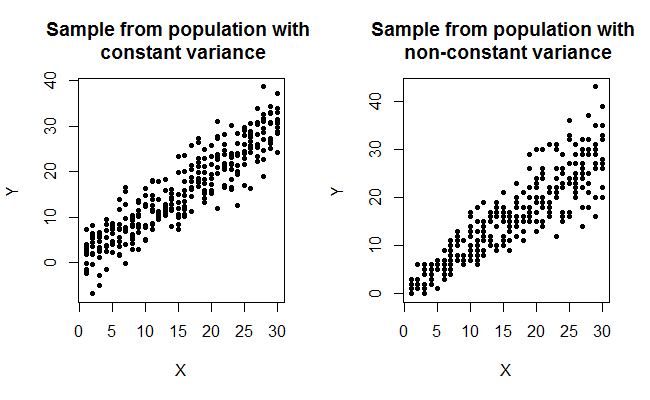
\includegraphics{hetero.png}

\end{frame}

\begin{frame}{A3c) Constant variance (homoskedasticity) errors}

\textbf{What happens if we violate this assumption?}

If we use model-based standard errors, then these will give incorrect
inference (i.e.~confidence intervals may not properly cover the true
\(\beta\)).

If we use robust standard errors, then we're okay!

\textbf{What can we do about it?}

Use robust standard errors! (\texttt{regress} uses these by default
while \texttt{lm} does not!)

\end{frame}

\begin{frame}{A4) Full rank predictor matrix}

\textbf{What does this mean?}

A matrix \(X\) is ``full rank'' if none of its columns are
\alert{collinear}.

In other words, we cannot have two columns \(X_1\) and \(X_2\) which can
be written as \(X_1 = aX_2 + b\) (e.g.~age in months and age in years).
Why might this be an issue, intuitively?

\pause

\textbf{What happens if we violate this assumption?}

Let's see what happens if we try to fit a model with collinear
predictors.

\end{frame}

\begin{frame}[fragile]{A4) Full rank predictor matrix}

\tiny

\begin{Shaded}
\begin{Highlighting}[]
\CommentTok{# Generate data}
\NormalTok{x1 =}\StringTok{ }\KeywordTok{rnorm}\NormalTok{(}\DecValTok{100}\NormalTok{)}
\NormalTok{x2 =}\StringTok{ }\DecValTok{2}\NormalTok{*x1 +}\StringTok{ }\DecValTok{3}
\NormalTok{y =}\StringTok{ }\DecValTok{2}\NormalTok{*x1 -}\StringTok{ }\NormalTok{x2 +}\StringTok{ }\KeywordTok{rnorm}\NormalTok{(}\DecValTok{100}\NormalTok{)}
\CommentTok{# Fit linear regression model}
\NormalTok{m =}\StringTok{ }\KeywordTok{lm}\NormalTok{(y ~}\StringTok{ }\NormalTok{x1 +}\StringTok{ }\NormalTok{x2)}
\KeywordTok{summary}\NormalTok{(m)}
\end{Highlighting}
\end{Shaded}

\begin{verbatim}
## 
## Call:
## lm(formula = y ~ x1 + x2)
## 
## Residuals:
##     Min      1Q  Median      3Q     Max 
## -2.3357 -0.5840 -0.1529  0.6968  1.9717 
## 
## Coefficients: (1 not defined because of singularities)
##             Estimate Std. Error t value Pr(>|t|)    
## (Intercept) -3.18840    0.08948 -35.633   <2e-16 ***
## x1           0.01941    0.09968   0.195    0.846    
## x2                NA         NA      NA       NA    
## ---
## Signif. codes:  0 '***' 0.001 '**' 0.01 '*' 0.05 '.' 0.1 ' ' 1
## 
## Residual standard error: 0.8944 on 98 degrees of freedom
## Multiple R-squared:  0.0003867,  Adjusted R-squared:  -0.009813 
## F-statistic: 0.03791 on 1 and 98 DF,  p-value: 0.846
\end{verbatim}

\normalsize

\end{frame}

\begin{frame}{A4) Full rank predictor matrix}

We cannot fit regression coefficients for all collinear variables!

If variables are strongly, but not perfectly correlated, coefficients
can still be fit. However, stronger correlation will lead to larger
standard errors, adding more uncertainty to inference.

\pause
\textbf{What can we do about it?}

Including very strongly correlated variables doesn't really make sense,
as we are repeating information. It's better to screen out variables
which are not really necessary.

Fortunately, we can easily look at pairwise correlations in our observed
data.

\end{frame}

\begin{frame}{A4) Full rank predictor matrix}

Another situation that results in a non-full rank \(X\) matrix is when
the number of variables, \(p > n\), the number of observations
(\alert{high-dimensional}).

In this situation, ordinary linear regression models cannot be fit; we
need to add more constraints to the model in order to obtain parameter
estimates.

If interested in this area, talk to Brian!!!

\end{frame}

\begin{frame}{Recap}

What do we \textit{actually} need?

\pause

\begin{itemize}
\tightlist
\item
  Independent observations
\item
  Robust standard errors
\item
  \(n\) sufficiently large; in particular, \(n >> p\)
\item
  Predictors are not strongly correlated
\item
  A model specification that is \textit{close enough} to the ground
  truth
\end{itemize}

\end{frame}

\begin{frame}{Diagnostics}

Can we test if our model assumptions are met?

\pause

Kind of. Diagnostics are a sanity check to see if your model is
\alert{terrible} or not.

\pause

What diagnostics do NOT do:

\begin{itemize}
\tightlist
\item
  Identify all possible issues in a model
\item
  Provide reliable \alert{model selection} criteria
\end{itemize}

\end{frame}

\begin{frame}{Residuals}

After fitting a regression model, the \alert{residuals} for each
observation are defined as
\(r_i = y_i - \sum_{i=0}^p \hat{\beta}_i x_i\) \centering
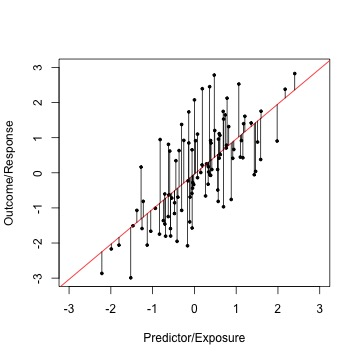
\includegraphics{linear-regr-ls.jpg}

\end{frame}

\begin{frame}{Residual plots}

Why do we consider the regression residuals for diagnostics?

\pause

The residuals are our ``best guess'' for the distribution of the
\(\epsilon_i\), which a lot of the regression assumptions involve.

\pause

The most common plot for linear regression diagnostics is a scatterplot
of residuals vs. \alert{fitted values} (defined as
\(\sum_{i=0}^p \hat{\beta}_i x_i\)).

\end{frame}

\begin{frame}{Residuals vs.~fitted values}

What we look for in this plot:

\begin{itemize}
\tightlist
\item
  Residuals spread randomly around the \(y = 0\) --\textgreater{}
  \(\epsilon\) zero mean
\item
  No ``trend'' in the residuals --\textgreater{} \(\epsilon\)
  independent of \(X\)
\item
  Constant height between min and max residuals at each level of fitted
  values --\textgreater{} constant variance
\end{itemize}

\end{frame}

\begin{frame}[fragile]{Residuals vs.~fitted values}

\tiny

\begin{Shaded}
\begin{Highlighting}[]
\NormalTok{x1 =}\StringTok{ }\KeywordTok{rnorm}\NormalTok{(}\DecValTok{100}\NormalTok{)}
\NormalTok{x2 =}\StringTok{ }\KeywordTok{c}\NormalTok{(}\KeywordTok{rep}\NormalTok{(}\DecValTok{1}\NormalTok{, }\DecValTok{50}\NormalTok{), }\KeywordTok{rep}\NormalTok{(}\DecValTok{2}\NormalTok{,}\DecValTok{50}\NormalTok{))}
\NormalTok{epsilon =}\StringTok{ }\KeywordTok{rnorm}\NormalTok{(}\DecValTok{100}\NormalTok{) }\CommentTok{# constant error variance}
\NormalTok{y =}\StringTok{ }\DecValTok{3} \NormalTok{+}\StringTok{ }\FloatTok{0.3}\NormalTok{*x1 +}\StringTok{ }\FloatTok{1.5}\NormalTok{*x2 +}\StringTok{ }\NormalTok{epsilon}
\NormalTok{m =}\StringTok{ }\KeywordTok{lm}\NormalTok{(y ~}\StringTok{ }\NormalTok{x1 +}\StringTok{ }\NormalTok{x2)}
\KeywordTok{plot}\NormalTok{(}\KeywordTok{fitted}\NormalTok{(m), }\KeywordTok{residuals}\NormalTok{(m), }\DataTypeTok{xlab =} \StringTok{"Fitted values"}\NormalTok{, }\DataTypeTok{ylab =} \StringTok{"Residuals"}\NormalTok{, }\DataTypeTok{pch=}\DecValTok{19}\NormalTok{)}
\KeywordTok{abline}\NormalTok{(}\DataTypeTok{h=}\DecValTok{0}\NormalTok{)}
\end{Highlighting}
\end{Shaded}

\includegraphics{biost311lecture_files/figure-beamer/unnamed-chunk-4-1.pdf}

\normalsize

\end{frame}

\begin{frame}[fragile]{Residuals vs.~fitted values}

\tiny

\begin{Shaded}
\begin{Highlighting}[]
\NormalTok{x1 =}\StringTok{ }\KeywordTok{rnorm}\NormalTok{(}\DecValTok{100}\NormalTok{)}
\NormalTok{x2 =}\StringTok{ }\KeywordTok{c}\NormalTok{(}\KeywordTok{rep}\NormalTok{(}\DecValTok{1}\NormalTok{, }\DecValTok{50}\NormalTok{), }\KeywordTok{rep}\NormalTok{(}\DecValTok{2}\NormalTok{,}\DecValTok{50}\NormalTok{))}
\NormalTok{epsilon =}\StringTok{ }\KeywordTok{c}\NormalTok{(}\KeywordTok{rnorm}\NormalTok{(}\DecValTok{50}\NormalTok{), }\KeywordTok{rnorm}\NormalTok{(}\DecValTok{50}\NormalTok{, }\DataTypeTok{sd =} \FloatTok{0.1}\NormalTok{)) }\CommentTok{# non-constant error variance}
\NormalTok{y =}\StringTok{ }\DecValTok{3} \NormalTok{+}\StringTok{ }\FloatTok{0.3}\NormalTok{*x1 +}\StringTok{ }\FloatTok{1.5}\NormalTok{*x2 +}\StringTok{ }\NormalTok{epsilon}
\NormalTok{m =}\StringTok{ }\KeywordTok{lm}\NormalTok{(y ~}\StringTok{ }\NormalTok{x1 +}\StringTok{ }\NormalTok{x2)}
\KeywordTok{plot}\NormalTok{(}\KeywordTok{fitted}\NormalTok{(m), }\KeywordTok{residuals}\NormalTok{(m), }\DataTypeTok{xlab =} \StringTok{"Fitted values"}\NormalTok{, }\DataTypeTok{ylab =} \StringTok{"Residuals"}\NormalTok{, }\DataTypeTok{pch=}\DecValTok{19}\NormalTok{, }\DataTypeTok{col =} \NormalTok{x2)}
\KeywordTok{abline}\NormalTok{(}\DataTypeTok{h=}\DecValTok{0}\NormalTok{)}
\end{Highlighting}
\end{Shaded}

\includegraphics{biost311lecture_files/figure-beamer/unnamed-chunk-5-1.pdf}

\normalsize

\end{frame}

\begin{frame}[fragile]{Residuals vs.~fitted values}

\tiny

\begin{Shaded}
\begin{Highlighting}[]
\CommentTok{# Generate data}
\NormalTok{x1 =}\StringTok{ }\KeywordTok{rnorm}\NormalTok{(}\DecValTok{100}\NormalTok{)}
\NormalTok{x2 =}\StringTok{ }\KeywordTok{c}\NormalTok{(}\KeywordTok{rep}\NormalTok{(}\DecValTok{1}\NormalTok{, }\DecValTok{50}\NormalTok{), }\KeywordTok{rep}\NormalTok{(}\DecValTok{2}\NormalTok{,}\DecValTok{50}\NormalTok{))}
\NormalTok{epsilon =}\StringTok{ }\KeywordTok{rnorm}\NormalTok{(}\DecValTok{100}\NormalTok{) }
\NormalTok{y =}\StringTok{ }\DecValTok{3} \NormalTok{+}\StringTok{ }\KeywordTok{exp}\NormalTok{(}\DecValTok{2}\NormalTok{*x1) +}\StringTok{ }\FloatTok{1.5}\NormalTok{*x2 +}\StringTok{ }\NormalTok{epsilon}
\CommentTok{# Fit linear regression with misspeccified model}
\NormalTok{m =}\StringTok{ }\KeywordTok{lm}\NormalTok{(y ~}\StringTok{ }\NormalTok{x1)}
\KeywordTok{plot}\NormalTok{(}\KeywordTok{fitted}\NormalTok{(m), }\KeywordTok{residuals}\NormalTok{(m), }\DataTypeTok{xlab =} \StringTok{"Fitted values"}\NormalTok{, }\DataTypeTok{ylab =} \StringTok{"Residuals"}\NormalTok{, }\DataTypeTok{pch=}\DecValTok{19}\NormalTok{)}
\KeywordTok{abline}\NormalTok{(}\DataTypeTok{h=}\DecValTok{0}\NormalTok{)}
\end{Highlighting}
\end{Shaded}

\includegraphics{biost311lecture_files/figure-beamer/unnamed-chunk-6-1.pdf}

\normalsize

\end{frame}

\begin{frame}{Residual Q-Q plot}

A Q-Q (quantile-quantile) plot compares two distributions by plotting
their quantiles against each other. The distributions are equal if the
resulting scatterplot goes through the 45-degree diagonal line

We use Normal Q-Q plots of residuals to judge if the model errors are
normally distributed.

\end{frame}

\begin{frame}[fragile]{Residual Q-Q plot}

\tiny

\begin{Shaded}
\begin{Highlighting}[]
\NormalTok{x1 =}\StringTok{ }\KeywordTok{rnorm}\NormalTok{(}\DecValTok{1000}\NormalTok{)}
\NormalTok{x2 =}\StringTok{ }\KeywordTok{c}\NormalTok{(}\KeywordTok{rep}\NormalTok{(}\DecValTok{1}\NormalTok{, }\DecValTok{500}\NormalTok{), }\KeywordTok{rep}\NormalTok{(}\DecValTok{2}\NormalTok{,}\DecValTok{500}\NormalTok{))}
\NormalTok{epsilon =}\StringTok{ }\KeywordTok{rnorm}\NormalTok{(}\DecValTok{1000}\NormalTok{)}
\NormalTok{y =}\StringTok{ }\DecValTok{3} \NormalTok{+}\StringTok{ }\FloatTok{0.3}\NormalTok{*x1 +}\StringTok{ }\FloatTok{1.5}\NormalTok{*x2 +}\StringTok{ }\NormalTok{epsilon}
\NormalTok{m =}\StringTok{ }\KeywordTok{lm}\NormalTok{(y ~}\StringTok{ }\NormalTok{x1 +}\StringTok{ }\NormalTok{x2)}
\KeywordTok{qqnorm}\NormalTok{(}\KeywordTok{residuals}\NormalTok{(m)) }\CommentTok{# QQ-plot comparing residuals to N(0,1) distribution}
\KeywordTok{abline}\NormalTok{(}\DecValTok{0}\NormalTok{,}\DecValTok{1}\NormalTok{)}
\end{Highlighting}
\end{Shaded}

\includegraphics{biost311lecture_files/figure-beamer/unnamed-chunk-7-1.pdf}

\normalsize

\end{frame}

\begin{frame}[fragile]{Residual Q-Q plot}

\tiny

\begin{Shaded}
\begin{Highlighting}[]
\NormalTok{x1 =}\StringTok{ }\KeywordTok{rnorm}\NormalTok{(}\DecValTok{1000}\NormalTok{)}
\NormalTok{x2 =}\StringTok{ }\KeywordTok{c}\NormalTok{(}\KeywordTok{rep}\NormalTok{(}\DecValTok{1}\NormalTok{, }\DecValTok{500}\NormalTok{), }\KeywordTok{rep}\NormalTok{(}\DecValTok{2}\NormalTok{,}\DecValTok{500}\NormalTok{))}
\NormalTok{epsilon =}\StringTok{ }\KeywordTok{rnorm}\NormalTok{(}\DecValTok{1000}\NormalTok{, }\DataTypeTok{sd =} \DecValTok{3}\NormalTok{) }\CommentTok{# Still normal, but no longer with variance = 1}
\NormalTok{y =}\StringTok{ }\DecValTok{3} \NormalTok{+}\StringTok{ }\FloatTok{0.3}\NormalTok{*x1 +}\StringTok{ }\FloatTok{1.5}\NormalTok{*x2 +}\StringTok{ }\NormalTok{epsilon}
\NormalTok{m =}\StringTok{ }\KeywordTok{lm}\NormalTok{(y ~}\StringTok{ }\NormalTok{x1 +}\StringTok{ }\NormalTok{x2)}
\KeywordTok{qqnorm}\NormalTok{(}\KeywordTok{residuals}\NormalTok{(m)) }\CommentTok{# QQ-plot comparing residuals to N(0,1) distribution}
\KeywordTok{abline}\NormalTok{(}\DecValTok{0}\NormalTok{,}\DecValTok{1}\NormalTok{)}
\end{Highlighting}
\end{Shaded}

\includegraphics{biost311lecture_files/figure-beamer/unnamed-chunk-8-1.pdf}

\normalsize

\end{frame}

\begin{frame}[fragile]{Residual Q-Q plot}

\tiny

\begin{Shaded}
\begin{Highlighting}[]
\NormalTok{x1 =}\StringTok{ }\KeywordTok{rnorm}\NormalTok{(}\DecValTok{1000}\NormalTok{)}
\NormalTok{x2 =}\StringTok{ }\KeywordTok{c}\NormalTok{(}\KeywordTok{rep}\NormalTok{(}\DecValTok{1}\NormalTok{, }\DecValTok{500}\NormalTok{), }\KeywordTok{rep}\NormalTok{(}\DecValTok{2}\NormalTok{,}\DecValTok{500}\NormalTok{))}
\NormalTok{epsilon =}\StringTok{ }\KeywordTok{rnorm}\NormalTok{(}\DecValTok{1000}\NormalTok{, }\DataTypeTok{sd =} \DecValTok{3}\NormalTok{) }\CommentTok{# Still normal, but no longer with variance = 1}
\NormalTok{y =}\StringTok{ }\DecValTok{3} \NormalTok{+}\StringTok{ }\FloatTok{0.3}\NormalTok{*x1 +}\StringTok{ }\FloatTok{1.5}\NormalTok{*x2 +}\StringTok{ }\NormalTok{epsilon}
\NormalTok{m =}\StringTok{ }\KeywordTok{lm}\NormalTok{(y ~}\StringTok{ }\NormalTok{x1 +}\StringTok{ }\NormalTok{x2)}
\KeywordTok{qqnorm}\NormalTok{(}\KeywordTok{stdres}\NormalTok{(m)) }\CommentTok{# QQ-plot comparing *standardized* residuals to N(0,1) distribution}
\KeywordTok{abline}\NormalTok{(}\DecValTok{0}\NormalTok{,}\DecValTok{1}\NormalTok{)}
\end{Highlighting}
\end{Shaded}

\includegraphics{biost311lecture_files/figure-beamer/unnamed-chunk-9-1.pdf}

\normalsize

\end{frame}

\begin{frame}{Residual ACF plot}

The ACF (autocorrelation function) plot displays the empirical
correlation of all observations separated by various time lags. For
randomly sampled data with no natural ordering of the observations, we
would expect these correlations to be small and non-significant.

We can look at the autocorrelation of the residuals to determine if the
independent \(\epsilon\) assumption holds. This might be a good idea if
we are less aware of how the data were generated, and there is the
possiblity of correlated observations.

\end{frame}

\begin{frame}[fragile]{Residual ACF plot}

\tiny

\begin{Shaded}
\begin{Highlighting}[]
\NormalTok{x1 =}\StringTok{ }\KeywordTok{rnorm}\NormalTok{(}\DecValTok{1000}\NormalTok{)}
\NormalTok{x2 =}\StringTok{ }\KeywordTok{c}\NormalTok{(}\KeywordTok{rep}\NormalTok{(}\DecValTok{1}\NormalTok{, }\DecValTok{500}\NormalTok{), }\KeywordTok{rep}\NormalTok{(}\DecValTok{2}\NormalTok{,}\DecValTok{500}\NormalTok{))}
\NormalTok{epsilon =}\StringTok{ }\KeywordTok{rnorm}\NormalTok{(}\DecValTok{1000}\NormalTok{)}
\NormalTok{y =}\StringTok{ }\DecValTok{3} \NormalTok{+}\StringTok{ }\FloatTok{0.3}\NormalTok{*x1 +}\StringTok{ }\FloatTok{1.5}\NormalTok{*x2 +}\StringTok{ }\NormalTok{epsilon}
\NormalTok{m =}\StringTok{ }\KeywordTok{lm}\NormalTok{(y ~}\StringTok{ }\NormalTok{x1 +}\StringTok{ }\NormalTok{x2)}
\KeywordTok{acf}\NormalTok{(}\KeywordTok{resid}\NormalTok{(m), }\DataTypeTok{lag.max=}\DecValTok{10}\NormalTok{) }
\end{Highlighting}
\end{Shaded}

\includegraphics{biost311lecture_files/figure-beamer/unnamed-chunk-10-1.pdf}

\normalsize

\end{frame}

\begin{frame}{Summary of diagnostics}

\begin{itemize}
\tightlist
\item
  By examining a residuals vs.~fitted values plot, we can determine if
  we have a serious model misspecification issue (if we just have
  non-constant variance, this is less of a big deal with large enough
  \(n\))
\item
  A Q-Q plot of the standardized residuals can tell us if the normality
  of residuals assumption is justifiable (but this is also less of a big
  deal with large enough \(n\))
\item
  The residual ACF plot can be useful if we think there is a possiblity
  of correlated data, in which case standard linear regression would not
  work out
\end{itemize}

\end{frame}

\end{document}
